\documentclass[tikz,border=8pt]{standalone}
\usepackage{amsmath}
\usetikzlibrary{arrows.meta,calc}

\begin{document}
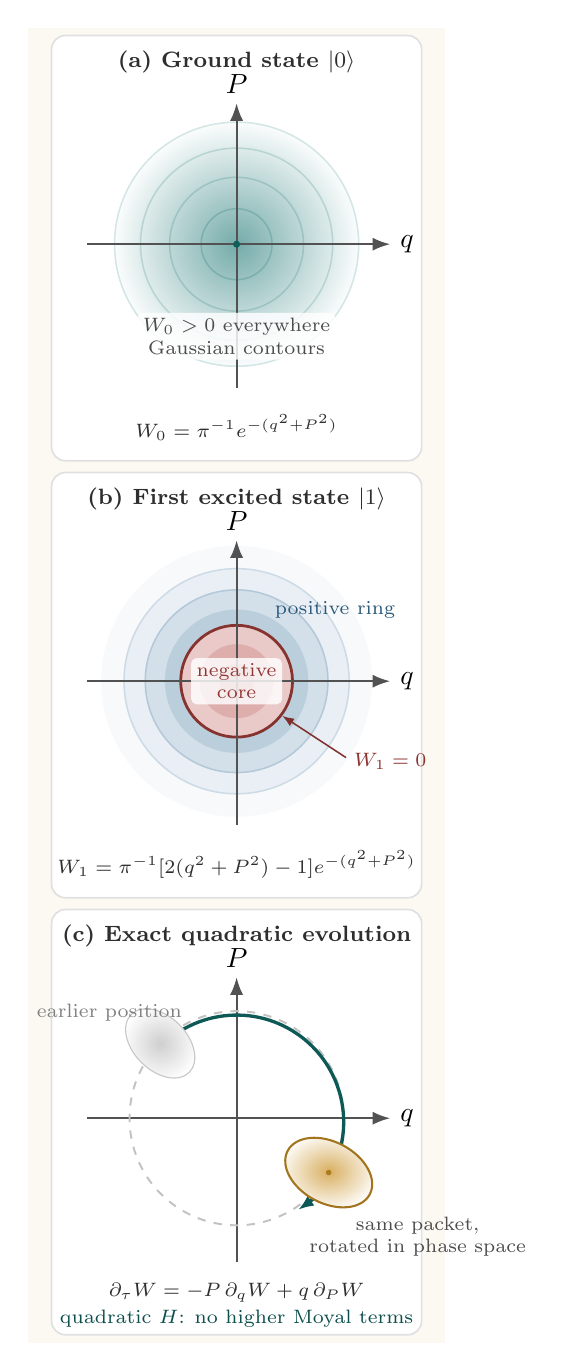
\begin{tikzpicture}[
  >=Latex,
  font=\sffamily,
  axis/.style={->, line width=.75pt, draw=black!68},
  contour/.style={line width=.55pt},
  paneltitle/.style={font=\footnotesize\bfseries, text=black!82, align=center},
  note/.style={font=\scriptsize, text=black!70, align=center},
  equation/.style={font=\scriptsize, text=black!82, align=center}
]

\definecolor{paper}{RGB}{252,249,243}
\definecolor{teal}{RGB}{16,111,108}
\definecolor{blue}{RGB}{54,111,153}
\definecolor{red}{RGB}{176,67,62}
\definecolor{gold}{RGB}{202,145,37}

\fill[paper] (-2.65,-8.35) rectangle (2.65,8.35);

\foreach \cy in {5.55,0,-5.55}{
  \fill[white,rounded corners=5pt]
    (-2.35,\cy-2.70) rectangle (2.35,\cy+2.70);
  \draw[black!12,rounded corners=5pt,line width=.6pt]
    (-2.35,\cy-2.70) rectangle (2.35,\cy+2.70);
}

% Ground-state Gaussian
\begin{scope}[shift={(0,5.55)}]
  \node[paneltitle] at (0,2.36) {(a) Ground state $\lvert0\rangle$};

  \shade[inner color=teal!58,outer color=teal!2]
    (0,.05) circle (1.55);
  \draw[contour,teal!55] (0,.05) circle (.45);
  \draw[contour,teal!42] (0,.05) circle (.85);
  \draw[contour,teal!30] (0,.05) circle (1.22);
  \draw[contour,teal!18] (0,.05) circle (1.55);

  \draw[axis] (-1.90,.05) -- (1.95,.05) node[right] {$q$};
  \draw[axis] (0,-1.78) -- (0,1.84) node[above] {$P$};

  \fill[teal!85!black] (0,.05) circle (.045);
  \node[note,fill=white,fill opacity=.82,text opacity=1,rounded corners=2pt,
    inner sep=2pt] at (0,-1.12)
    {$W_0>0$ everywhere\\Gaussian contours};
  \node[equation] at (0,-2.28)
    {$W_0=\pi^{-1}e^{-(q^2+P^2)}$};
\end{scope}

% First excited state: negative core, positive ring
\begin{scope}[shift={(0,0)}]
  \node[paneltitle] at (0,2.36) {(b) First excited state $\lvert1\rangle$};

  \fill[blue!4] (0,.05) circle (1.72);
  \fill[blue!11] (0,.05) circle (1.43);
  \fill[blue!22] (0,.05) circle (1.16);
  \fill[blue!34] (0,.05) circle (.91);
  \fill[red!28] (0,.05) circle (.71);
  \fill[red!43] (0,.05) circle (.47);
  \fill[red!62] (0,.05) circle (.22);

  \draw[contour,blue!38] (0,.05) circle (1.16);
  \draw[contour,blue!25] (0,.05) circle (1.43);
  \draw[red!76!black,line width=1pt] (0,.05) circle (.71);

  \draw[axis] (-1.90,.05) -- (1.95,.05) node[right] {$q$};
  \draw[axis] (0,-1.78) -- (0,1.84) node[above] {$P$};

  \node[note,text=red!82!black,fill=white,fill opacity=.82,text opacity=1,
    rounded corners=2pt,inner sep=2pt] at (0,.05) {negative\\core};
  \node[note,text=blue!80!black] at (1.25,.96) {positive ring};
  \draw[-{Latex[length=1.5mm]},red!72!black,line width=.55pt]
    (1.39,-.92) -- (.58,-.39);
  \node[note,anchor=west,text=red!78!black] at (1.37,-.97)
    {$W_1=0$};
  \node[equation] at (0,-2.28)
    {$W_1=\pi^{-1}[2(q^2+P^2)-1]e^{-(q^2+P^2)}$};
\end{scope}

% Exact harmonic flow: displaced Gaussian rotates clockwise
\begin{scope}[shift={(0,-5.55)}]
  \node[paneltitle] at (0,2.36) {(c) Exact quadratic evolution};

  \draw[axis] (-1.90,.05) -- (1.95,.05) node[right] {$q$};
  \draw[axis] (0,-1.78) -- (0,1.84) node[above] {$P$};

  \draw[black!24,dashed,line width=.7pt] (0,.05) circle (1.36);
  \draw[-{Latex[length=2mm]},teal!80!black,line width=1.2pt]
    (145:1.36) arc[start angle=145,end angle=-55,radius=1.36];

  \begin{scope}[shift={(-.97,1.00)},rotate=-45]
    \shade[inner color=black!19,outer color=white]
      (0,0) ellipse (.52 and .34);
    \draw[black!22] (0,0) ellipse (.52 and .34);
  \end{scope}

  \begin{scope}[shift={(1.17,-.64)},rotate=-28]
    \shade[inner color=gold!72,outer color=gold!4]
      (0,0) ellipse (.59 and .39);
    \draw[gold!80!black,line width=.75pt] (0,0) ellipse (.59 and .39);
    \fill[gold!85!black] (0,0) circle (.035);
  \end{scope}

  \node[note,anchor=west] at (.80,-1.45)
    {same packet,\\rotated in phase space};
  \node[note,anchor=east,text=black!50] at (-.57,1.39)
    {earlier position};
  \node[equation] at (0,-2.16)
    {$\partial_\tau W=-P\,\partial_qW+q\,\partial_PW$};
  \node[equation,text=teal!70!black] at (0,-2.49)
    {quadratic $H$: no higher Moyal terms};
\end{scope}

\end{tikzpicture}
\end{document}
